%\documentclass[draft,reqno,T1]{amsart}
\documentclass[aps,english,superscriptaddress,twocolumn,twoside,prl]{revtex4-1}%
\usepackage[paperwidth=210mm,paperheight=297mm,centering,hmargin=2cm,vmargin=2.5cm]{geometry}
\usepackage[usenames,dvipsnames]{color}
\usepackage{tikz}
\usetikzlibrary{arrows,automata,petri,shapes,positioning,circuits.ee.IEC}
\definecolor{ultramarine}{RGB}{63, 0, 255}
\definecolor{medblue}{RGB}{0, 0, 100}
\definecolor{panblue}{RGB}{0,24,150}
\definecolor{carmine}{RGB}{150, 0, 24}
\definecolor{gray}{RGB}{150, 150, 150}
\usepackage{amssymb}
\usepackage{amsmath}
\usepackage{amsfonts}
\usepackage{amsthm}
\usepackage{geometry}
\usepackage{bbm}
\usepackage{mathrsfs}
\usepackage{pbox}
\usepackage[tight]{subfigure}
\usepackage{multirow}
\usepackage[makeroom]{cancel}
\usepackage{braket} %provide \bra and \Bra and \set and \Set etc...
\usepackage[first=0,last=1]{lcg} % provides \rand
\usepackage{siunitx} % provides \num

\usepackage{verbatim} %for comment command
\usepackage{microtype}

\usepackage{mathtools} %for mathclap and prescript and more. Learning to love this package. And DeclarePairDelimeter!
\DeclarePairedDelimiter\ceil{\lceil}{\rceil}
\DeclarePairedDelimiter\floor{\lfloor}{\rfloor}

% commutative diagrams
\usepackage[all]{xy}

% internal links should be highlighted in blue 
\definecolor{myurlcolor}{rgb}{0,0,0.4}
\definecolor{mycitecolor}{rgb}{0,0.5,0}
\definecolor{myrefcolor}{rgb}{0.5,0,0}
\usepackage[pagebackref,colorlinks,draft=false]{hyperref}
\hypersetup{linkcolor=myrefcolor,citecolor=carmine,urlcolor=panblue,anchorcolor=OliveGreen}
\renewcommand*{\backref}[1]{$\uparrow$\,#1}

% macros
\newcommand{\beq}{\begin{equation}}
\newcommand{\eeq}{\end{equation}}
\newcommand{\Z}{\mathbb{Z}}
\newcommand{\C}{\mathbb{C}}
\newcommand{\N}{\mathbb{N}}
\newcommand{\Q}{\mathbb{Q}}
\newcommand{\R}{\mathbb{R}}
\newcommand{\F}{\mathbb{F}}
\newcommand{\Rplus}{\mathbb{R}_{\geq 0}}
\renewcommand{\H}{\mathcal{H}}
\renewcommand{\O}{\mathcal{O}}
\newcommand{\M}{\mathcal{M}}
\newcommand{\B}{\mathcal{B}}
\newcommand{\K}{\mathcal{K}}
\renewcommand{\S}{\mathcal{S}}
\newcommand{\ra}{\rightarrow}
\newcommand{\lra}{\longrightarrow}
\newcommand{\eps}{\varepsilon}
\newcommand{\supp}{\mathrm{supp}}
\newcommand{\cone}{\mathrm{cone}}
\newcommand{\lsa}{\leftsquigarrow}
\newcommand{\rsa}{\rightsquigarrow}
\newcommand{\lin}{\mathrm{lin}}
\newcommand{\tr}{\mathrm{tr}}
\newcommand{\id}{\mathrm{id}}
\newcommand{\T}[1]{\texttt{#1}}
\newcommand{\defin}{:=}
\newcommand{\disjcup}{\stackrel{\cdot}{\cup}} % notation for disjoint union
\newcommand{\indf}[1]{\mathbbm{1}_{#1}} % indicator function
\newcommand{\blank}{\underline{\hspace{6pt}}} % placeholder symbol

% causal structure stuff
\newcommand{\src}[1]{{\mathrm{src}(#1)}}
\newcommand{\tar}[1]{{\mathrm{tar}(#1)}}
\newcommand{\pa}[1]{{\mathrm{pa}(#1)}}
\newcommand{\ch}[1]{{\mathrm{ch}(#1)}}
\newcommand{\pst}[1]{{\mathrm{pst}(#1)}}
\newcommand{\pste}[1]{{\mathrm{pst}^+(#1)}}
\newcommand{\inc}[1]{{\mathrm{in}(#1)}}
\newcommand{\out}[1]{{\mathrm{out}(#1)}}

% categories
\newcommand{\Cp}{\mathtt{C}}
\newcommand{\Dp}{\mathtt{D}}
\newcommand{\Pp}{\mathtt{C_1}}
\newcommand{\Qp}{\mathtt{D_1}}
\newcommand{\sop}{\mathtt{StOp}}
\newcommand{\fsop}{\mathtt{FinStOp}}
\renewcommand{\sp}{\mathtt{StOp_1}}
\newcommand{\qop}{\mathtt{QOp}}
\newcommand{\FinStoch}{\mathtt{FinStoch}}
\newcommand{\ground}{
\begin{tikzpicture}[thick,scale=.8,circuit ee IEC] \node[ground,rotate=90]{}; \end{tikzpicture}} % ground symbol as morphism to terminal object

% Theorem Environments
%\swapnumbers
\theoremstyle{plain}
\newtheorem{thm}{Theorem}%[section]
\newtheorem{lem}[thm]{Lemma}
\newtheorem{prop}[thm]{Proposition}
\newtheorem{cor}[thm]{Corollary}
\newtheorem{conj}[thm]{Conjecture}
\newtheorem{qstn}[thm]{Question}
\newtheorem*{utheorem}{Theorem}
\newtheorem*{ulemma}{Lemma}
\newtheorem*{uprop}{Proposition}
\newtheorem*{ucor}{Corollary}
\newtheorem{defn}[thm]{Definition}
\newtheorem{prob}[thm]{Problem}
\newtheorem*{udefn}{Definition}
\theoremstyle{definition}
\newtheorem{expl}[thm]{Example}
\newtheorem*{uexample}{Example}
\theoremstyle{remark}
\newtheorem{rem}[thm]{Remark}
\newtheorem{note}[thm]{Note}
\newtheorem*{uremark}{Remark}
\newtheorem*{unote}{Note}
\numberwithin{equation}{section}
\newenvironment{partialproof}{\paragraph{\textsc{Partial Proof.}}}{\hfill$\square$\bigskip}
\newenvironment{sketchproof}{\paragraph{\textsc{Sketch of Proof.}}}{\hfill$\square$\bigskip}

%%%%%%%%%%%% Enumeration via lowercase letters
\renewcommand{\labelenumi}{(\alph{enumi})}
\renewcommand{\theenumi}{(\alph{enumi})}
\renewcommand{\labelitemi}{$\circ$}

%%% pagebreaks allowed for align environment
\allowdisplaybreaks

%%% emphasis
\renewcommand{\emph}[1]{\textbf{#1}}
\newcommand{\emphalt}[1]{\textit{#1}}

% vertical spacing in multiline equations
\setlength{\jot}{6pt}

%-------------------------------------------------------------------

%%%Use normal equations numbers considering no sections - Elie
\renewcommand{\theequation}{\arabic{equation}}

\newcommand{\na}{\ensuremath{\mathring{a}}}
\newcommand{\nb}{\ensuremath{\mathring{b}}}
\newcommand{\nc}{\ensuremath{\mathring{c}}}
%\newcommand{\notb}[2]{\reflectbox{b}}



\usepackage{mathtools} %for mathclap and prescript and more. Learning to love this package. And DeclarePairDelimeter!
%\DeclarePairedDelimiter\ceil{\lceil}{\rceil}
%\DeclarePairedDelimiter\floor{\lfloor}{\rfloor}
%-------------------------------------------------------------------

\begin{document}
%\sloppy



%%%%%%%%%%%% title page stuff %%%%%%%%%%%%%%%%%%%%%%%%%%

\title[]{Some inequalities for the triangle scenario}

\author{Tobias Fritz}
\affiliation{Perimeter Institute for Theoretical Physics\\ Waterloo, Ontario, Canada, N2L 2Y5}
\email{tfritz@perimeterinstitute.ca}

%\keywords{}

%\subjclass[2010]{Primary: ; Secondary: }

\thanks{
%\hspace*{-\parskip}\noindent\textsc{\textsc{Acknowledgements}}\hspace{\parskip} 
Research at Perimeter Institute is supported by the Government of Canada through Industry Canada and by the Province of Ontario through the Ministry of Economic Development and Innovation. The author has been supported by the John Templeton Foundation.}

\begin{abstract}
I sketch the derivation of some inequalities that hold for classical correlations in the triangle scenario.
\end{abstract}

\maketitle
\onecolumngrid
I present several inequalities for binary outcomes together with a method of proof which has a combinatorial flavour. No quantum violations of any of these inequalities has been found to date.

In the following the complement of a value is marked by an empty circle accent, so $\mathring{b}$ means ``anything but $b$", and accordingly $P(\mathring{a}\mathring{b})=P(A\mathopen{\neq}a,B\mathopen{\neq}b)$. Additionally, an underscore stands for the corresponding marginal probability, like this: $P(\_b\_)\defin P(abc) + P(ab\mathring{c}) + P(\mathring{a}bc) + P(\mathring{a}b\mathring{c})$. 
\begin{thm}
The following inequalities hold for all classical correlations in the triangle scenario:
\begin{enumerate}
\item
\(\quad
P(a) P(c)  \leq  P(ab) + P(\nb c)
\)
\item
\(\quad
%P(001) P(010) P(100)  \leq  P(000) + P(11\_) P(001) P(0\_\_) + P(1\_1) P(010) P(\_\_0) + P(\_11) P(100) P(\_0\_)
P(a b\nc) P(a \nb c) P(\na b c) \leq P(a b c) + P(\na \nb) P(a b \nc) P(a) + P(\na\nc) P(a\nb c) P(c)  + P(\nb \nc) P(\na b c) P(b)
\)
\item 
\(\quad
P(001) P(010) P(100) \leq  P(000)^2 + 2 P(11\_) P(001) + 2 P(1\_1) P(010)
+ 2 P(\_11) P(100)
\)
\item
\(\quad
P(000)^2 P(111)  \leq  P(001) P(010) P(100) + (2 P(000) + P(111)) (1 -
P(000) - P(111))
\)
\item
\(\quad
P(000)^2 P(111)  \leq  P(000)^3 + (2 P(000) + P(111)) (1 - P(000) - P(111))
\)
\item
\(\quad
P(a) P(b) P(c) \leq  P(\na\nb\nc) + P(a b) P(c) + P(a c) P(b) + P(b c) P(a)
\)
\item
\(\quad
P(a) P(b) P(c) \leq  P(\na\nb\nc)^2 +2\left( P(a b) P(c) + P(a c) P(b) + P(b c) P(a) \right)
\)
\end{enumerate}
\end{thm}

It is quite likely that some of these inequalities are dominated by the others, but I do not know for sure whether any of them are actually redundant.

\begin{proof}
We reduce the problem to counting cycles in a graph as follows.

The classical correlations are precisely those that can be written in the form
\[
P(abc) = \sum_{\mathclap{\lambda_{AB},\lambda_{BC},\lambda_{AC}}} P(a|\lambda_{AB}\lambda_{AC}) P(b|\lambda_{AB}\lambda_{BC}) P(c|\lambda_{BC}\lambda_{AC}) P(\lambda_{AB}) P(\lambda_{BC}) P(\lambda_{AC}).
\]
By a suitable fine-graining, we can approximate such a classical model arbitrarily well by another one in which the hidden variables are uniformly distributed on a finite set $\Lambda$,
\beq
\label{uniform}
P(abc) = \sum_{\mathclap{\lambda_{AB},\lambda_{BC}\lambda_{AC}}} P(a|\lambda_{AB}\lambda_{AC}) P(b|\lambda_{AB}\lambda_{BC}) P(c|\lambda_{BC},\lambda_{AC}).
\eeq
Hence it is sufficient to prove the inequalities for all distributions of this form. Moreover, we may assume without loss of generality that all response functions are deterministic, i.e.~$P(a|\lambda_{AB}\lambda_{AC})\in\{0,1\}$
%$P(a,b|\lambda_3)\in\{0,1\}$
, etc. In this way, the right-hand side of~\eqref{uniform} simply counts the number of triples for which each conditional probability takes on the value $1$, so that
\[
P(abc) = \left|\set{ (\lambda_{AB},\lambda_{BC}\lambda_{AC}) \: |\: P(a|\lambda_{AB}\lambda_{AC}) = P(b|\lambda_{AB}\lambda_{BC}) = P(c|\lambda_{BC},\lambda_{AC}) = 1 } \right|\cdot |\Lambda|^{-3},
\]
where the factor of $|\Lambda|^{-3}$ now is the probability of each triple of hidden variable values $(\lambda_{AB},\lambda_{BC}\lambda_{AC})$ to occur. Since all our inequalities can be made homogeneous (see below), we can simply omit this constant scalar factor. So it is sufficient to prove that the numbers
\beq
\label{cyclecounter}
N(abc) = \left|\set{ (\lambda_{AB},\lambda_{BC}\lambda_{AC}) \: |\: P(a|\lambda_{AB}\lambda_{AC}) = P(b|\lambda_{AB}\lambda_{BC}) = P(c|\lambda_{BC},\lambda_{AC}) = 1 } \right|%\cdot |\Lambda|^{-3}
,
\eeq
in place of $P(a,b,c)$ satisfy our inequalities.

\begin{figure}
\centering
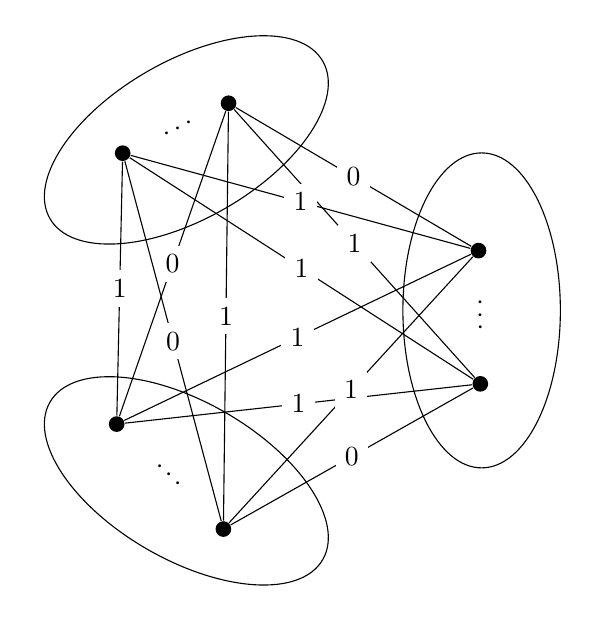
\begin{tikzpicture}
	\def\separ{2.5}
	\def\randx{rand*.3}
	\def\randy{rand*.3}
	\tikzstyle{vertex} = [circle,fill,inner sep=2pt]
	\foreach \i in {1,...,3}{
		\begin{scope}[rotate=120*\i]
		\draw (\separ,0) ellipse (1cm and 2cm) coordinate (center\i);
		\foreach \n in {0,1}{
			\node[vertex] (node\i\n) at ($(\separ,0)+(\randx,\randy+\n*1.8-.9)$) {} ; }
		\draw[draw=none] (node\i0) -- (node\i1) node [midway,sloped,anchor=center,rotate=120*\i] {$\cdots$} ;
		\end{scope}}
	\foreach \i in {1,...,3} \foreach \j in {1,...,3} {
		\def\labeling{\pgfmathparse{int(round(rand/2+.5))}\pgfmathresult}
		\ifthenelse{\i<\j}{\foreach \n in {0,1} \foreach \m in {0,1} \draw (node\i\n) -- (node\j\m) node [midway,fill=white] {\labeling};}{} }
\end{tikzpicture}
\caption{Illustration of the labelled graph constructed in the proof.}
\label{fig:graph}
\end{figure}

But now these numbers can be understood in terms of cycles on graphs: as illustrated in Figure~\ref{fig:graph}, we consider the complete tripartite graph with one vertex for each possible value of each hidden variable $\lambda_i$. The edge between two hidden variable values $\lambda_2$ and $\lambda_3$ is labelled by the corresponding conditional probability $P(a|\lambda_2,\lambda_3)$, and similarly for $P(b|\lambda_3,\lambda_1)$ and $P(c|\lambda_1,\lambda_2)$. Then~\eqref{cyclecounter} counts nothing but the number of $3$-cycles in this graph whose edge labels are precisely the outcomes $a$, $b$ and $c$ under consideration. With this in mind, the following arguments are all of the same form: for any cycle contributing to the left-hand side, there will be a corresponding cycle contributing to the right-hand side. The inequality then follows if the map from the left-hand side cycles to the right-hand side cycles is injective, since it follows that the cardinality of the former set is bounded by the cardinality of the latter. Now on to the various cases:


\begin{figure}[h]
\centering
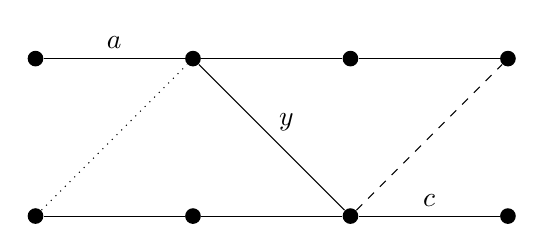
\begin{tikzpicture}
	\def\xsep{2}
	\def\ysep{1}
	\foreach \x in {0,...,3} \foreach \y in {-1,1} \node[fill,inner sep=2pt,circle] (node\x\y) at (\x*\xsep,\y*\ysep) {};
	\draw (node01) -- node [midway,above] {$a$} (node11) -- (node21) -- (node31) ;
	\draw (node0-1) -- (node1-1) -- (node2-1) -- node [midway,above] {$c$} (node3-1) ;
	\draw (node11) -- (node2-1) node [pos=.6,above=4pt] {$y$} ;
	\draw[dashed] (node2-1) -- (node31) ;
	\draw[dotted] (node0-1) -- (node11) ;
\end{tikzpicture}
\caption{Illustration of the proof of~\eqref{firstineq}. In order for a sensible drawing to be possible, the cyclic structure of Figure~\ref{fig:graph} has now been cut open into a linear structure, so that each vertex on the right end is actually equal to the corresponding vertex on the left end.}
\label{fig:aillu}
\end{figure}
\begin{enumerate}
\item In homogeneous form, we need to show
\beq
\label{firstineq}
N(a\_\_) N(\_\_c) \leq N(ab\_) N(\_\_\_) + N(\_\nb c) N(\_\_\_).
\eeq
To see this, consider Figure~\ref{fig:aillu}: the left-hand side of the inequality counts all pairs of cycles for which the first edge in the first cycle is labelled $a$ and the third edge in the second cycle by $c$. For any such pair, we consider the label $y$ in Figure~\ref{fig:aillu}: if it is $b$, then we obtain a cycle with labels $ab?$ by taking $a$, $y$ and then the dashed edge, and one with completely unknown labels $???$ by taking the complementary path. But if $y=\nb$, then we can obtain a cycle $?\mathring{b}c$ by taking the dashed edge first, together with a cycle $???$ with completely unknown labels. Since these cases contribute to different terms on the right-hand side of~\eqref{firstineq}, we obtain the desired injective map.

\begin{comment}
\item In homogeneous form, this inequality says
\begin{align}
\begin{split}
\label{secondineqOLD}
 N(001) N(010) N(100) \leq & N(000) N(\_\_\_) N(\_\_\_) \\
 & + N(11\_) N(001) N(0\_\_) \\
 & + N(1\_1) N(010) N(\_\_0) \\
 & + N(\_11) N(100) N(\_0\_) .
\end{split}
\end{align}
The proof is similar to the previous one; again we start with the left-hand side, which now counts triples of cycles with labels $001$, $010$ and $100$ as illustrated as the horizontal lines in Figure~\ref{fig:billu}. Now consider the labels of the dashed edges $x$, $y$ and $z$. If $x=y=z=0$, then we choose this cycle and rewire the rest in an arbitrary manner, resulting in a contribution to the first term on the right-hand side. Otherwise, at least one of $x$, $y$ or $z$ is equal to $1$; suppose $y=1$. Then we choose the cycle $1y?$ starting and ending at the bottom vertices, keep the top $001$ one, which leaves a unique choice of $0??$ for the third cycle; this gives a contribution to the second term. The other cases where $x=1$ or $z=1$ are analogous.
\begin{figure}[h]
\centering
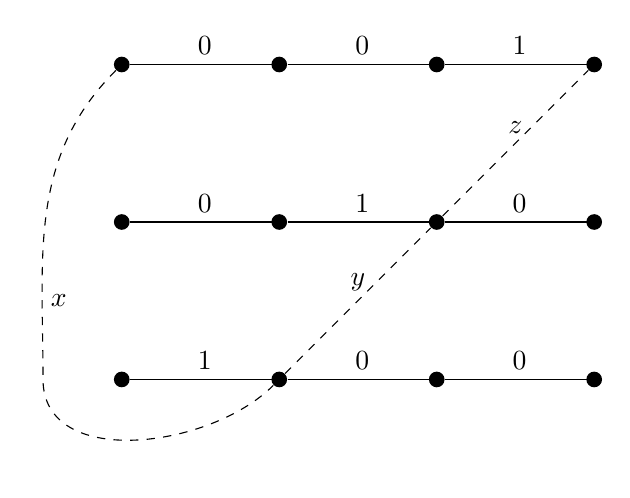
\begin{tikzpicture}
	\def\xsep{2}
	\def\ysep{2}
	\foreach \x in {0,...,3} \foreach \y in {0,...,2} \node[fill,inner sep=2pt,circle] (node\x\y) at (\x*\xsep,\y*\ysep) {};
	\foreach \x in {0,...,2} \foreach \y in {0,...,2} \draw (node\x\y) -- node[midway,above] {$\pgfmathparse{equal(\x,\y)}\pgfmathresult$} ($(node\x\y)+(\xsep,0)$) ;
	\draw[dashed] (node02) to [out=-135,in=90] (-1,0)  to [out=-90,in=-135] (node10) ;
	\node at (-.8,1) {$x$} ;
	\draw[dashed] (node10) -- (node21) node [midway,above] {$y$} ;
	\draw[dashed] (node21) -- (node32) node [midway,above] {$z$} ;
\end{tikzpicture}
\caption{Illustration of the proof of~\eqref{secondineq}.}
\label{fig:billuOLD}
\end{figure}
\end{comment}

\item In homogeneous form, this inequality says
\begin{align}
\begin{split}
\label{secondineq}
 N(a b\nc) N(a \nb c) N(\na b c) \leq & N(abc) N(\_\_\_) N(\_\_\_) \\
 & + N(\na \nb\_) N(a b \nc) N(a\_\_) \\
 & + N(\na\_\nc) N(a\nb c) N(\_\_c) \\
 & + N(\_\nb \nc) N(\na b c) N(\_b\_) .
\end{split}
\end{align}
The proof is similar to the previous one; again we start with the left-hand side, which now counts triples of cycles with labels $a b\nc$, $a \nb c$ and $\na b c$ as illustrated as the horizontal lines in Figure~\ref{fig:billu}. Now consider the labels of the dashed edges $x$, $y$ and $z$. If $x=a,y=b,z=c$, then we choose this cycle and rewire the rest in an arbitrary manner, resulting in a contribution to the first term on the right-hand side. Otherwise, at least one of $x$, $y$ or $z$ corresponds to a complimentary value; suppose $y=\nb$. Then we choose the cycle $\na y ?$ starting and ending at the bottom vertices, keep the top $a b \nc$ one, which leaves a unique choice of $a??$ for the third cycle; this gives a contribution to the second term. The other cases where $x=\na$ or $z=\nc$ are analogous.
\begin{figure}[h]
\centering
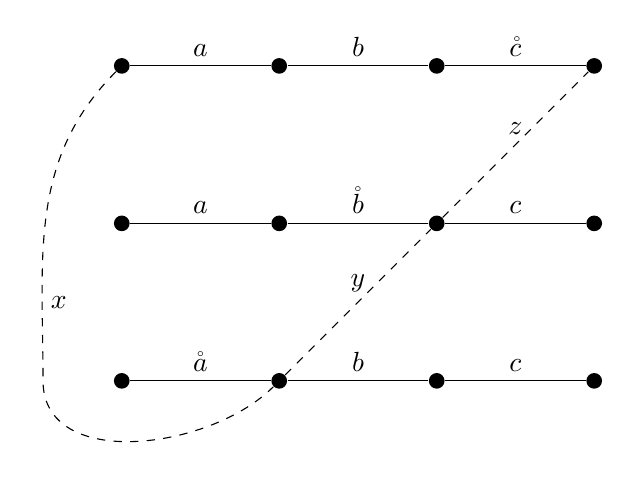
\begin{tikzpicture}
	\def\xsep{2}
	\def\ysep{2}
	\foreach \x in {0,...,3} \foreach \y in {0,...,2} \node[fill,inner sep=2pt,circle] (node\x\y) at (\x*\xsep,\y*\ysep) {};
%	\foreach \x in {0,...,2} \foreach \y in {0,...,2} \draw (node\x\y) -- node[midway,above] {$\pgfmathparse{equal(\x,\y)}\pgfmathresult$} ($(node\x\y)+(\xsep,0)$) ;
\draw (node00) -- (node10)  node [midway,above] {$\na$} ;
\draw (node10) -- (node20)  node [midway,above] {$b$} ;
\draw (node20) -- (node30)  node [midway,above] {$c$} ;
\draw (node01) -- (node11)  node [midway,above] {$a$} ;
\draw (node11) -- (node21)  node [midway,above] {$\nb$} ;
\draw (node21) -- (node31)  node [midway,above] {$c$} ;
\draw (node02) -- (node12)  node [midway,above] {$a$} ;
\draw (node12) -- (node22)  node [midway,above] {$b$} ;
\draw (node22) -- (node32)  node [midway,above] {$\nc$} ;
\draw[dashed] (node02) to [out=-135,in=90] (-1,0)  to [out=-90,in=-135] (node10) ;
	\node at (-.8,1) {$x$} ;
	\draw[dashed] (node10) -- (node21) node [midway,above] {$y$} ;
	\draw[dashed] (node21) -- (node32) node [midway,above] {$z$} ;
\end{tikzpicture}
\caption{Illustration of the proof of~\eqref{secondineq}.}
\label{fig:billu}
\end{figure}

\item \dots The proofs of all other inequalities should be similar\dots\qedhere
\end{enumerate}
\end{proof}


\end{document}


%%%% old inequalities dominated by other ones

\item 
\[
P(001) P(010) P(100) \leq  P(000) + P(11\_) P(001) + P(1\_1) P(010) +
P(\_11) P(100)
\]
